\section{Java}
Java je jedním z nejpoužívanějších a nejpopulárnějších počítačových programovacích jazyků na světě. Syntaxe tohoto jazyka se řadí k těm jednodužším, avšak jeho použití je velmi rozsáhlé. V Java se programují čipové karty, mobilní a desktopové aplikace, i velké podnikové a informační systémy. Java je jazyk multiplatformní a díky tomu je jej možné použít ná různých operačních systémech. Java je vyvíjena jako OpenSource. Java se objevuje ve třech základních edicích:


\subsection{Java platformy}
Jazyk Java je společně s virtuálním strojem a knihovnami vydáván ve čtyřech platformách, kde každá má své speciální určení.

\subsubsection{Java SE}
Základní platforma pro vývoj desktopových a jednodužších serverových aplikací. V součané době je poslední vydaná verze Java SE 8u25.

\subsubsection{Java EE}
Nádstavba nad Java SE obsahující speciální knihovny pro vývoj a provoz podnikových aplikací a informačních systémů. V součané době je poslední vydaná verze Java EE 7.

\subsubsection{Java ME (Micro Edition)}
Podmnožina Java SE pro vývoj aplikací pro malá zařízení jako jsou mikrokontroléry sensory, mobilní telefony, set-top boxy, tiskárny a další. V součané době je poslední vydaná verze Java ME 8.1.

\subsubsection{Java Card}
Verze určená pro vývoj aplikací určených pro čipové karty a pro zařízení s limitovanou pamětí a schopností zpracovávání. Příkladem mohou být SIM karty pro mobilní zařízení nebo čipové karty pro ATM bankomaty. V součané době je poslední vydaná verze Java Card 3.0.4.

\subsection{Vývojářské sady}
Možnosti jak Javu stáhnout jsou dvě. Jedná se o balík se kterým lze pouze spouštět aplikace Java (JRE) nebo balík který slouží pro vývoj (JDK).

\subsubsection{Java JRE (Java Runtime Environment)}
Běhové prostředí Javy, které poskytuje vše potřebné pro suštění java aplikací. Součástí je virtuální stroj javy a potřebné knihovny.

\subsubsection{Java JDK (Java Development Kit)}
Někdy se také označuje SDK (Software Development Kit). Jedná se o sadu JRE doplněnou o vyvojářské nástroje (překladač, generátor dokumentace, ladící nástroje a další).

\begin{figure}[h!]
    \centering
    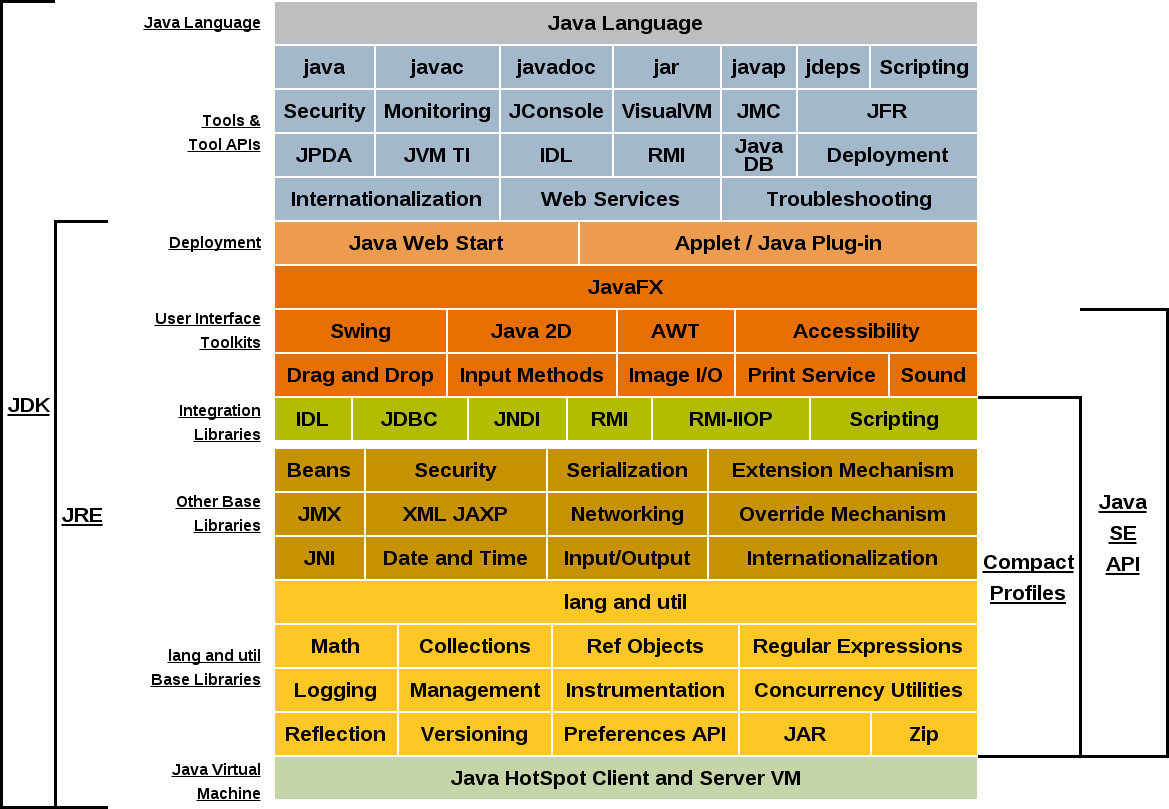
\includegraphics[scale=0.3]{fig/java_jdk.jpg}
    \caption{Java SE JDK 1.8}
\end{figure}



\section{Android}
Android je mobilní operační systém vyvíjený společností Google, který je založený na Linuxovém jádře. Je vyvíjen jako opensource a používá se především v mobilních zařízeních jako jsou chytré telefony, hodinky a tablety. Můžeme jej však také nalézt také v přístrojích jako jsou set-top boxy, multimediální přehrávače a v jiné elektronice.\\
\subsection{Historie}
Počátky Androidu spadají do roku 2003, kdy byla v Kalifornii v USA založena společnost Android, Inc. O Dva roky později firmu odkupuje světoznámá společnost Google. V roce 2007 získává Google několik patentů v oblasti mobilních zařízení a 5. listopadu téhož roku dochází k oficiálnímu představení a vzniká sdružení firem Open Handset Alliance, která mé za cíl vytvoření otevřených standartů v oblasti mobilních zařízení. V tabulce TODO odkaz je zobrazena stručná historie verzí operačního systému Android.

\begin {table}[h!]
\begin{tabular}{|l|c|l|c|}
\hline
{\bf Datum}         & {\bf Verze}   & {\bf Označení}        & {\bf Verze API}   \\
\hline \hline
23. září 2008       & 1.0 -- 1.1    & --                    & 1 -- 2            \\
\hline
April 27, 2009      & 1.5           & Cupcake               & 3                 \\
\hline
September 15, 2009  & 1.6           & Donut                 & 4                 \\
\hline
October 26, 2009    & 2.0 -- 2.1    & Eclair                & 5 -- 7            \\
\hline
May 20, 2010        & 2.2 -- 2.2.3  & Froyo                 & 8                 \\
\hline
December 6, 2010    & 2.3 -- 2.3.7  & Gingerbread           & 9 -- 10           \\
\hline
February 22, 2011   & 3.0 -- 3.2    & Honeycomb             & 11 -- 13          \\
\hline
October 18, 2011    & 4.0 -- 4.0.4  & Ice Cream Sandwich    & 14 -- 15          \\
\hline
July 9, 2012        & 4.1 -- 4.3    & Jelly Bean            & 16 -- 18          \\
\hline
October 31, 2013    & 4.4           & KitKat                & 19 -- 20          \\
\hline
November 12, 2014   & 5.0           & Lollipop              & 21                \\
\hline
\end{tabular}
\centering
\caption{Verze operačního systému Android}
\end{table}

\subsection{Arcitektura}
Architektura systému android je složena z šesti vrstev:
\begin{itemize}
\item Linuxové jádro
\item HAL
\item Knihovny
\item Android runtime
\item Application framework
\item Aplikace
\end{itemize}
\subsubsection{Linuxové jádro}
Tato nejnižší vrstva je postavena mezi hardware zařízení a ostatní vrstvy architektury. Od počátku byl android postaven na jádru 2.6, nejnověší android pak běží na jádru 3.4. Při startu se jádro zavede do operační paměti a je mu předáno řízení.
\subsubsection{HAL}
TODO
\subsubsection{Knihovny}
Nad linuxovým jádrem se nachází vrstva knihoven obsahující open source webový prohlížeč Webkit, knihovnu libc TODO
\subsubsection{Android runtime}
TODO
\subsubsection{Application framework}
Vrstva aplikačního frameworku poskytuje mnoho vysoko-úrovňových služeb aplikacím ve formě java knihoven. Pro vývojáře se jedná o nejdůležitější vrstvu,která umožňuje přístup ke službám daného zařízení. Tato vrstva je tvořena: 
\begin{itemize}
\item Activity manager -- ovládání životního cyklu aplikací
\item Windows manager
\item Content manager 
\item View system -- 
\item Notification manager --
\item Package manager -- 
\item Telephony manager
\item Resource manager
\item Location manager
\item a další...
\end{itemize}
TODO

\subsubsection{Aplikace}
Poslední a nejvyšší vrstva se skládá ze samotných aplíkací. Jendak se jedná o předinstalované aplikace a druhak se jedná o aplikace, které byly postupem času přidány z android obchodu nebo jinou cestou.

\begin{figure}[h!]
    \centering
    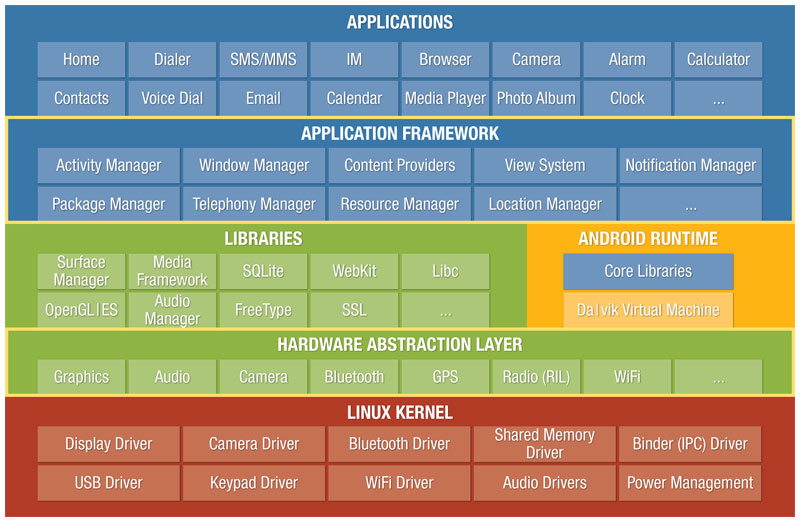
\includegraphics[scale=0.5]{fig/android_architecture.jpg}
    \caption{Java SE JDK 1.8}
\end{figure}

\section{Gradle}


\section{JBoss Drools}

  \subsection{Drools Expert}

  \subsection{OptaPlanner}


\section{Vehicle routing problem}

%\subsection{History}
%V následující tabulce je stručně popsána historie programovacího jazyku Java: \\
%\\
%\begin {table}[h!]
%\begin{tabular}{|l|l|l|}[h]
%\hline
%    {\bf Název} & {\bf Datum} & {\bf Poznámka}  \\
%    \hline \hline
%    Oak         & 1991                  & a     \\
%    JDK         & 1995                  & a     \\
%    JDK 1.0     & January 23rd, 1996    & a     \\
%    JDK 1.1     & February 19th, 1997   & a     \\
%    JPE         & May, 1998             & a \\
%    J2SE 1.2    & December 8th, 1998    & a     \\
%    J2EE 1.2    & December 12, 1999     & a     \\
%    J2SE 1.3    & May 8th, 2000         & a     \\
%    J2EE 1.3    & September 24, 2001    & a \\
%    J2SE 1.4    & February 6th, 2002    & a     \\
%    J2EE 1.4    & November 11, 2003     & a \\
%    J2SE 5.0    & September 30th, 2004  & a     \\
%    Java EE 5   & May 11, 2006          & a \\
%    Java SE 6   & December 11th, 2006   & a     \\
%    Java EE 6   & December 10, 2009     & a \\
%    Java SE 7   & July 28th, 2011       & a     \\
%    Java EE 7   & June 12, 2013         & a \\
%    Java SE 8   & March 18th, 2014      & a     \\
%  \hline
%\end{tabular}
%\caption{Historie Javy}
%\end{table}




